\documentclass[11pt]{article}
\usepackage{deauthor,times,graphicx,url} 


%% \newlength{\bibitemsep}\setlength{\bibitemsep}{.2\baselineskip plus .05\baselineskip minus .05\baselineskip}
%% \newlength{\bibparskip}\setlength{\bibparskip}{0pt}
%% \let\oldthebibliography\thebibliography
%% \renewcommand\thebibliography[1]{%
%%   \oldthebibliography{#1}%
%%   \setlength{\parskip}{\bibitemsep}%
%%   \setlength{\itemsep}{\bibparskip}%
%% }
%% \setlength{\bibitemsep}{.1\baselineskip plus .05\baselineskip minus .05\baselineskip}



\newcommand{\squishlist}{
 \begin{list}{$\bullet$}
  { \setlength{\itemsep}{0pt}
     \setlength{\parsep}{1pt}
     \setlength{\topsep}{1pt}
     \setlength{\partopsep}{0pt}
     \setlength{\leftmargin}{1.5em}
     \setlength{\labelwidth}{1em}
     \setlength{\labelsep}{0.5em} } }
 \newcommand{\squishend}{\end{list}}


\begin{document}
\title{Entities with Quantities} %5-8 pages
\author{Gerhard Weikum\\Max Planck Institute for Informatics\\Saarland Informatics Campus E1.4, Saarbr\"ucken, Germany\\weikum@mpi-inf.mpg.de}

%\maketitle


%\section*{The Web as a Database !?}
\subsection*{The Web as a Database }

Unstructured content, like text in web pages, and semistructured content, like HTML tables in web pages, has much weaker search functionality compared to structured databases. For example, joins between text documents via co-occurring entity mentions or attribute values are infeasible, unless major efforts are taken to create mark-up for a structured view. As for web tables, filters on entity mentions allow users to look up data, but results are noisy and 
error-prone because of ad-hoc choices for names of entities and value encodings, with huge heterogeneity across tables and often even within a table. 

In the last few years, large knowledge graphs (KG), 
machine learning (ML) techniques and advances in entity linking algorithms \cite{Mudgal:SIGMOD2018,Shen:TKDE2015}
have enabled search engines to overcome these issues, to a large degree \cite{Noy:CACM2019}.
By detecting entity mentions in web content and normalizing them onto KG entries, it has become possible to answer entity-centric queries about people, places and products almost as precisely and concisely as  a database query.
%As illustration of these impressive advances,
The following examples work with all major search engines and return
crisp entity-level answers:

%\vspace*{0.05cm}
\begin{center}
{\small
\begin{tabular}{|l|l|}\hline
Query & Results(s) \\ \hline
Height of the Eiffel Tower & 324 meters\\
highest building in Paris & Eiffel Tower\\
CEO of Amazon & Jeff Bezos\\
Bezos worth & 108.9 Billion USD\\
CEOs of IT companies &  Jeff Bezos, Sundar Pichai, Ginny Rometti, Zhang Yong, \dots\\ \hline
\end{tabular}
}
\end{center}

Search engines leverage look-ups in back-end knowledge graphs,
and run entity detection on both user inputs and page contents
to provide these answers.
It seems that entity-centric search on the web has become as easy and 
as effective as querying a structured and curated database!

The same methodologies, particularly, entity linking,
are also key to joining data for the same entity
across web tables and
within heterogeneous data lakes \cite{Lehmberg:PVLDB2017,Zhu:SIGMOD2019}.
%%%cite Halevy here as well ???


\subsection*{Quantity Queries}

On the disillusioning side, there is an interesting and challenging type of queries
that is underexplored and hardly supported:
searching with {\em quantities}: quantitative measures of entities
that capture financial, physical, technological or environmental properties.
Examples are: 
%\squishlist
a celebrity's personal wealth,
a company's quarterly revenue, 
 a car's energy consumption,
 a material's thermal conductivity, or
 the usual and maximal dosage of a medical drug.
%\squishend
%\noindent 
Quantities can be represented as
$\langle measure, value, unit \rangle$ triples,
such as $\langle height, 8848, meter \rangle$.
The units can be simple, such as meters, light-years, US dollars, Euros etc.,
with well-defined conversion rules between different units for the
same measure. But they can also be quite sophisticated such as
{\em kWh/100km} for a car's energy consumption or 
{\em W/(mK)}
for the thermal conductivity of materials,
with more complex conversion rules, e.g., between
kWh/100km and MPG (miles per gallon) for electric, hybrid and fuel-based cars.
Conversions often require context information, such as
date for currency conversions, or location for car properties
(incl. carbon footprint).
The International System of Units (SI) is a rich reference for
measures and conversions 
%({\small\tt en.wikipedia.org/wiki/International\_System\_of\_Units}).
({\small\url{https://en.wikipedia.org/wiki/International_System_of_Units}}).

Search engines perform well on looking up quantities for given entities, such as
retrieving the height of the Eiffel Tower. In this regard, quantity properties
are not different from other properties such as city or architect.
The pain point, however, is {\em finding} all entities (of a certain type) that
satisfy a {\em search condition for a quantity of interest},
for example, buildings taller than 500m or runners completing a marathon under 2:10h. 
With few exceptions where explicit lists are available, search engines
fall back to returning page links only.
%and leave further reading of these pages
%to the user. 
The following examples illustrate this disappointing behavior.


%\vspace*{0.05cm}
\begin{center}
{\small
\begin{tabular}{|p{5cm}|p{10cm}|}\hline
Query & Results(s) \\ \hline\hline
people worth 50 Billion USD & link to ``List of Americans by net worth - Wikipedia'' \\ \hline
\dots more than 50 Billion USD & links to pages such as
``Meet the world's 50 richest billionaires in 2019''\\ \hline
\dots between 10 and 50 Billion Euros & links to pages such as
``Inequality and Wealth Distribution in Germany'' \\ \hline
\end{tabular}
}
\end{center}

Search engines do not understand numbers and units (with a few exceptions
regarding dates and money, sometimes). For example, ``15 kW'' and
``15.000 W'' are two different strings.
Units like ``l/100km'', 
``MPG'', ``MPGe'' and ``kWh/100km'' are also just strings, and the systems are
%agnostic of the option for unit conversion.
ignorant about unit conversions.

These queries would be trivial to handle if all data resided
in a single database with well-designed schema,
standardized value encodings, and high-quality curation.
However, these databases do rarely exist, or are outdated or incomplete.
One would hope that this is where encyclopedic knowledge graphs
kick in, such as DBpedia, Wikidata or Yago.
However, quantitative properties are very sparse in these KGs,
and often represented just as strings, e.g., ``250 mi $\pm$ 10''
for the range of a car model.
Only Wikidata contains triples for the range of cars, but only for
4 models (as of Dec. 2019). 
As for other measures, like engine power, energy efficiency, carbon footprint etc.,
none of these KGs has any data.
% on such properties.
Only the Web as a whole contains the wealth of information that
is needed to compute accurate and complete answers to
many kinds of quantity queries.





%%%%%%%%%%%%%%%%%%%%%%%%%%%%%%%%%%%

\subsection*{Initial Proof of Concept}

Supporting quantity queries is easy over a 
single well-curated database. It is challenging over
web page contents, 
%and equally difficult over 
web table 
collections or data lakes.
%database federations.
%It is a daunting challenge when considering large data lakes,
%as they 
In the latter cases, we need to overcome the
obstacles of
highly heterogeneous schemas,
diverse and noisy value encodings, and widely varying degrees of
coverage \cite{Miller:DEbull2018}.
%\cite{Nargesian:PVLDB2018}.
%%%check if this is the best reference here
%(e.g., Open Data \cite{Nargesian:PVLDB2018}).

As an initial effort,
% in this research direction, 
we devised methods for
a limited class of quantity queries over text document collections such as
Wikipedia articles or news corpora. This work has led to an early
prototype system, called {\em Qsearch} \cite{Ho:ISWC2019,Ho:WSDM2020}.
The system consists of a {\em data preparation} stage with quantity extraction
and indexing, and a {\em query processing} stage with matching and ranking.
A Qsearch demonstrator is accessible at
{\small\url{https://qsearch.mpi-inf.mpg.de}}. 
Figure \ref{fig1-qsearch-screenshot} shows the top-ranked answers
for an example query about buildings higher than 1000 ft.

\begin{figure} [tb]
  \centering
   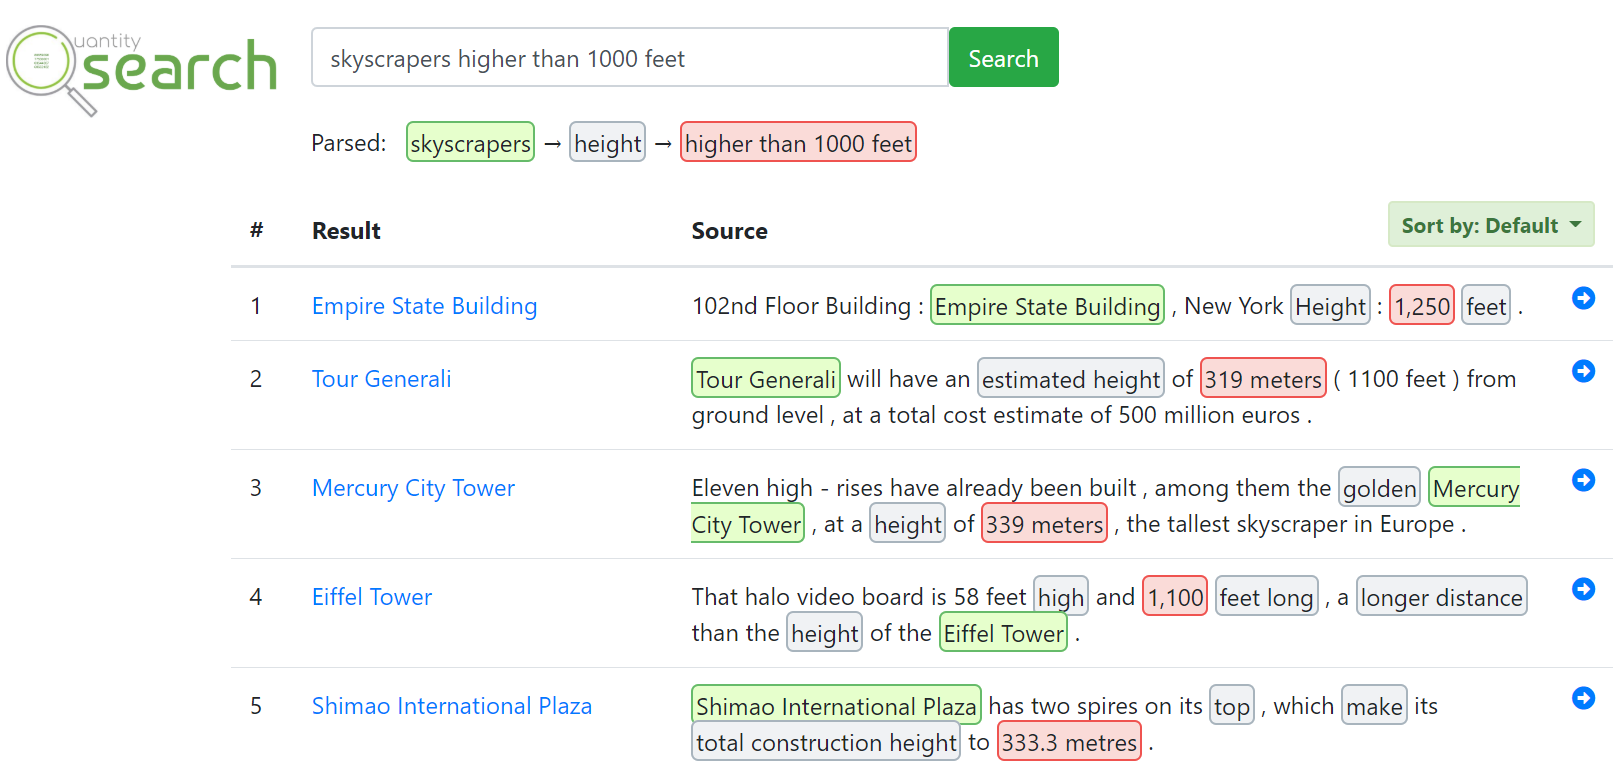
\includegraphics[width=0.8\textwidth]{letters/fig1-qsearch-screenshot.png}
\vspace*{-0.3cm} 
     \caption{Screenshot of Qsearch answers to query about buildings higher than 1000 ft}
      \label{fig1-qsearch-screenshot}
\end{figure}

\vspace{0.2cm}
\noindent{\bf Information Extraction:}
Qsearch 
%processes textual context one sentence at a time, using
uses
machine learning for sequence tagging. 
It trains an LSTM neural network with distant supervision,
and applies the learned model to tag each word in a sentence,
identifying three components:
i) an {\em entity} of interest, ii) a {\em quantity} that refers to this entity,
and iii) {\em context cues} that capture what exactly the quantity denotes.
For example, from the sentence
``The hybrid Prius is sold in Germany for less than 30 thousand, and
has a battery only range of 60 km.'',
Qsearch extracts two assertions:
first, related to price: i) Toyota Prius as key entity, 
ii) 30,000 Euros (upper bound) as quantity,
iii) ``sold in Germany'' as cue words,
and second, related to range: i) Toyota Prius as entity,
ii) 60 km as quantity, 
iii) ``battery only range'' as cue words.
%Entities are linked to a knowledge graph, this way canonicalizing their names,
%and quantities are normalized in a best-effort way, with units inferred when possible.
%All extracted assertions are indexed on all components.

\vspace{0.2cm}
\noindent{\bf Query Analysis:}
At query time, Qsearch analyzes telegraphic queries or full questions and 
decomposes them into three components:
{\em semantic target type} (e.g., buildings or hybrid cars etc.),
{\em quantity condition} of the form $\langle comparison, value, unit \rangle$
(with comparisons like $\le$, $\ge$, {between}, etc.),
{\em context cues} that candidate results should match (e.g., ``electric range in city traffic''
for a query about hybrid cars).

\vspace{0.2cm}
\noindent{\bf Matching and Ranking:}
Query processing aims to match all components of an assertion against the
components of the query: the entity must be of the right type,
the quantity condition must be satisfied, and the context cues must match
as well as possible (leveraging word embeddings, e.g., to capture the
relatedness of ``battery only'' and ``electric range'').
As the latter comes with uncertainty, Qsearch employs 
language-model-style ranking to compute the best answers.


%%%%%%%%%%%%%%%%%%%%%%%%%%%%%%%%


\subsection*{Challenges and Opportunities}

\noindent{\bf Quantity Filters:}
%
%extraction from text
Even basic filters over quantities still pose enormous challenges.
The extraction from text often faces complicated and misleading inputs, 
such as ``The battery of the hybrid Toyoto Prius lasts well over 100,000 miles''
as a spurious candidate for the electric range of this car.
For more sophisticated measures such as the CO2 footprint of cars, 
it is crucial to consider elaborate context like the source of energy for
electric cars, the driving situations (city vs. highway, summer vs. winter),
and more. This will rarely be fully captured in a single sentence;
so we need information extraction that combines and reconciles cues
from entire paragraphs or even multiple documents.
State-of-the-art work on quantity detection and extraction \cite{Alonso:SIGIR2018,Ho:ISWC2019,Ibrahim:CIKM2016,Roy:TACL2015,Saha:ACL2017,Sarawagi:KDD2014}
has disregarded such advanced settings so far.

%extraction from tables and open data
Major sources for quantity information are also web tables
and Open Data accessible on the Internet (e.g., 
{\small\tt www.data.gov}, {\small\tt data.gov.uk}, {\small\tt data.europa.eu},
%{\small\tt ec.europa.eu/eurostat/data/}, 
etc.).
Tapping into this kind of (semi-) structured web data comes with huge challenges.
Despite prior work on annotating cells in ad-hoc tables with entities and types
\cite{Bhagavatula:ISWC2015,Cafarella:PVLDB2018,Limaye:PVLDB2010,Venetis:PVLDB2011}, 
understanding quantities and their relations to entities in this kind of
online contents is way underexplored.
The most notable prior endeavor is the work of Sarawagi et al.~\cite{Sarawagi:KDD2014},
which focused on a limited range of query types over web tables.
Note that besides HTML tables in web pages, this direction should also consider 
spreadsheet data in enterprises as well as highly
% (if not wildly)
heterogeneous data lakes like Open Data.
In addition, combining tables with cues from their surrounding text
(in web pages or enterprise documents) could potentially be a powerful asset
\cite{Ibrahim:ICDE2019}.
%
%Leveraging all this 
%%rich (but fairly raw) 
%contents to aid analysts is a great research opportunity.


\vspace{0.2cm}
%\clearpage\newpage
\noindent{\bf Quantity Joins:}
A next step would be tackling comparisons between quantities, either
for the same entity or for different entities.
For example, we could ask for 100m sprinters whose best time in Olympics finals
is their personal record, or for such athletes whose time in the Olympics
was worse than their personal best of the same year.
These comparisons entail joins over the quantity values, in the second case
even a non-equi join.
The example may appear very special (of interest only to sports afficionados),
but similarly structured queries appear in other domains as well;
examples are comparing 
medical drugs and their usage 
%by various properties 
(e.g., 
%blood lab values 
%blood pressure medication
anti-coagulants
for which the 
%normal range 
standard dosage
is higher in the US than in the EU),
or environmental properties of fuel-based, hybrid and electric cars
in different geo-regions.

These queries are easy to express in SQL if the data resides in a single
high-quality database.
The challenge lies in applying them to extractions from text and tables
(incl. scientific literature such as PubMed, ClinicalTrials, etc.)
and to ad-hoc collections of many databases.

\vspace{0.2cm}
\noindent{\bf Quantity Aggregation:}
%
%already counting is difficult
%example olympic medals of Usain Bolt
%example olympic medals of German handball team
%
Given the inherent noise in extractions and the
incompleteness of tables, it is often necessary to aggregate 
quantity information from multiple sources.
For example, we may have to compute unions of entity sets
as a basis for grouping and aggregate comparisons,
or we have to combine many extractions
to approximate proper values.
% (using ML techniques).

Such aggregations can be amazingly difficult even for seemingly simple cases.
Already basic counting can be painful and challenging \cite{Mirza:ISWC2018}. 
Consider the example
of computing the total number of 
%Olympic and 
World Championship
medals that Usain Bolt has won in his career (answer is 14).
We may obtain cues from text and tables such as: 
he has won 100m three times,
he won 11 gold medals between 2009 and 2017,
he helped the Jamaican team to win the 4x100m relay race four times,
200m@2007 2nd place: Usain Bolt,
100m@2017 3rd place: Usain Bolt, etc.
Can we infer the total, or at least lower and upper bounds?
For prominent cases like Usain Bolt, this is not really necessary, as there
are high-quality tables and lists already 
%(e.g., in his Wikipedia article),
and we can look up the total rather than computing it.
However, for less popular entities, the accessible information is often partial
%(e.g., reporting only results for single events)
and spread across many sources.
One difficulty is to avoid over-counting by disregarding that the 11 gold medals
already include the four medals for the relay race.
If we first specified a rule system, about sports medals, we could use
reasoning to infer totals, but we want a solution that works out-of-the-box for
all possible domains. 
Can we use machine learning to predict bounds for totals and other aggregates,
with as little supervision as possible?

Obviously, the task gets only harder once we tackle quantities with units
for realistic use cases. For example, what are the average 
blood lab values
for diabetes patients of 
certain age groups in different parts of the world
(as reported in clinical studies at PubMed, and other online sources)?




%%%%%%%%%%%%%%%%%%%%%%%%%%%%%%%%

\subsection*{An Analyst's Dream}

%Why is 
%%all
% this valuable for mission-critical applications?
%Why 
%%should it be 
%is it
%interesting to the database
%%research
%community?
%% after all?

%Quantity queries have a small share in the user requests that search engines receive.
%However, 
Quantity queries are often part of high-stakes information needs by
advanced users, such as analysts, journalists, scientists
and other knowledge workers.
%In fact, they are a basic building block towards expressive data analytics
%over entities and their quantitative properties.
Ideally, an analyst would run her entire 
data analysis over web contents as easily as posing a keyword query or
single-sentence question:
\squishlist
\item Which runners have completed 10 marathons under 2 hours 10 minutes?
\item Which is the most energy-efficient hybrid car model? 
\item How does the carbon footprint of Japanese cars compare to US-made cars
when driven in the Bay Area?
%\item How much money does the UK save by leaving all EU research programs,
%as part of the Brexit?
\item Which 
%kinds of 
vaccinations have more than 80\% coverage in the 20 population-wise
largest countries?
\squishend
%Answering such queries by a search engine
%would be a breakthrough in boosting the productivity of content analysts.
%\noindent The goal is to support such tasks by search engines over
%web contents, including web tables. 
%The envisioned methodology should
%also help to get more value from highly heterogeneous data lakes
%(or combinations of web pages, web tables and online databases).
The envisioned solution should support search engines over textual contents,
web tables as well as heterogeneous data lakes.
% of Open Data.
The key issues of extracting, normalizing, matching, ranking and
aggregating quantities are the same regardless of whether we tap
into textual contents or structured but fairly raw data.

%%%GW: shorten this par
%Perhaps, quantity queries and analyses should 
%better be directed to
%structured data sources like knowledge graphs and online databases,
%not to search engines?
%Unfortunately, the required information is equally hard to find there, if not 
%harder. 
%Knowledge graphs such as Wikidata are very sparse in their coverage
%of quantities.
%Specialized databases have way more information, 
%but they are hard to discover in a huge and 
%highly heterogeneous ``data ocean'' (to re-position the term ``data lake'').
%In the end, without specific cues on where exactly the query should be
%directed, evaluating quantity queries over structured data on the Internet
%entails the same problems as posing them to a search engine.
%The key issues of extracting, normalizing, matching, ranking and
%aggregating quantities are the same regardless of whether we tap
%into textual contents of web pages or tables in data lakes!

%%%GW: just 1 or 2 sentences as final words
More than 30 years ago, 
%when the Web became popular as the ``Internet of contents'', 
%
%Tim Berners-Lee envisioned that the 
%...
%%% ... stated in his Turing Award speech ...
Bill Gates promised that ``all information is at your fingertips''
and Larry Page foresaw that ``the ultimate search engine would understand exactly
what you mean and give back exactly what you want''.
We have gone a long way towards these goals, but there are still
many obstacles.
% including the quantity-unawareness of search engines
%and the unsurmountable heterogeneity of data sources.
This opinion paper is a call to overcome these issues 
%at least for
%a limited but
for an interesting and valuable slice of information needs.

%“The ultimate search engine would understand exactly what you mean and give back exactly what you want.” Larry Page

%The web of human-readable document is being merged with a web of machine-understandable data
%https://www.w3.org/People/Berners-Lee/ShortHistory.html
%1998

%\newpage

\begin{thebibliography}{99} %0.5 pages
%limit to most important references, maybe 20

%{\normalsize

\bibitem{Alonso:SIGIR2018} Omar Alonso, Thibault Sellam:
Quantitative Information Extraction From Social Data. SIGIR 2018
%: 1005-1008

\bibitem{Bhagavatula:ISWC2015} Chandra Sekhar Bhagavatula, Thanapon Noraset, Doug Downey:
TabEL: Entity Linking in Web Tables. ISWC 2015
%: 425-441

\bibitem{Cafarella:PVLDB2018} Michael J. Cafarella, Alon Y. Halevy, Hongrae Lee, Jayant Madhavan, Cong Yu, Daisy Zhe Wang, Eugene Wu:
Ten Years of WebTables. PVLDB 11(12), 2018
%: 2140-2149 (2018)

\bibitem{Ho:ISWC2019} Vinh Thinh Ho, Yusra Ibrahim, Koninika Pal, Klaus Berberich, Gerhard Weikum:
Qsearch: Answering Quantity Queries from Text. ISWC 2019
%: 237-257

\bibitem{Ho:WSDM2020} Vinh Thinh Ho, Koninika Pal, Niko Kleer, Klaus Berberich, Gerhard Weikum:
Entities with Quantities: Extraction, Search, and Ranking.
Demo Paper, WSDM 2020

\bibitem{Ibrahim:CIKM2016} 	Yusra Ibrahim, Mirek Riedewald, Gerhard Weikum:
Making Sense of Entities and Quantities in Web Tables. CIKM 2016
%: 1703-1712


\bibitem{Ibrahim:ICDE2019} Yusra Ibrahim, Mirek Riedewald, Gerhard Weikum, Demetrios Zeinalipour-Yazti:
Bridging Quantities in Tables and Text. ICDE 2019
%: 1010-1021

\bibitem{Lehmberg:PVLDB2017} Oliver Lehmberg, Christian Bizer:
Stitching Web Tables for Improving Matching Quality. PVLDB 10(11), 2017
%: 1502-1513 (2017)

\bibitem{Limaye:PVLDB2010} Girija Limaye, Sunita Sarawagi, Soumen Chakrabarti:
Annotating and Searching Web Tables Using Entities, Types and Relationships. PVLDB 3(1), 2010
%: 1338-1347 (2010)


%\bibitem{Madaan:AAAI2016} Aman Madaan, Ashish Mittal, Mausam, Ganesh Ramakrishnan, Sunita Sarawagi:
%Numerical Relation Extraction with Minimal Supervision. AAAI 2016
%%: 2764-2771


\bibitem{Miller:DEbull2018} Renee J. Miller, Fatemeh Nargesian, Erkang Zhu, Christina Christodoulakis, Ken Q. Pu, Periklis Andritsos:
Making Open Data Transparent: Data Discovery on Open Data. IEEE Data Eng. Bull. 41(2), 2018
%: 59-70 (2018)


%\ bibitem{Mirza:ACL2017} Paramita Mirza, Simon Razniewski, Fariz Darari, Gerhard Weikum:
%Cardinal Virtues: Extracting Relation Cardinalities from Text. ACL 2017
%%: 347-351

\bibitem{Mirza:ISWC2018} Paramita Mirza, Simon Razniewski, Fariz Darari, Gerhard Weikum:
Enriching Knowledge Bases with Counting Quantifiers. 
%International Semantic Web Conference (1) 2018: 179-197
ISWC 2018


\bibitem{Mudgal:SIGMOD2018} Sidharth Mudgal, Han Li, Theodoros Rekatsinas, AnHai Doan, Youngchoon Park, Ganesh Krishnan, Rohit Deep, Esteban Arcaute, Vijay Raghavendra:
Deep Learning for Entity Matching: A Design Space Exploration. SIGMOD Conference 2018
%: 19-34

%\bibitem{Nargesian:PVLDB2018} Fatemeh Nargesian, Erkang Zhu, Ken Q. Pu, Renée J. Miller:
%Table Union Search on Open Data. PVLDB 11(7), 2018
%%: 813-825 (2018)

\bibitem{Noy:CACM2019} Natalya Fridman Noy, Yuqing Gao, Anshu Jain, Anant Narayanan, Alan Patterson, Jamie Taylor:
Industry-scale knowledge graphs: lessons and challenges. Commun. ACM 62(8), 2019
%: 36-43 (2019)


\bibitem{Roy:TACL2015} Subhro Roy, Tim Vieira, Dan Roth:
Reasoning about Quantities in Natural Language. TACL 3, 2015
%: 1-13 (2015)


\bibitem{Saha:ACL2017} Swarnadeep Saha, Harinder Pal, Mausam:
Bootstrapping for Numerical Open IE. ACL 2017
%: 317-323

\bibitem{Sarawagi:KDD2014} Sunita Sarawagi, Soumen Chakrabarti:
Open-domain quantity queries on web tables: annotation, response, and consensus models. KDD 2014
%: 711-720

\bibitem{Shen:TKDE2015} Wei Shen, Jianyong Wang, Jiawei Han:
Entity Linking with a Knowledge Base: Issues, Techniques, and Solutions. IEEE Trans. Knowl. Data Eng. 27(2),
%443-460 (2015)
2015

\bibitem{Venetis:PVLDB2011} Petros Venetis, Alon Y. Halevy, Jayant Madhavan, Marius Pasca, Warren Shen, Fei Wu, Gengxin Miao, Chung Wu:
Recovering Semantics of Tables on the Web. PVLDB 4(9), 2011
%: 528-538 (2011)

\bibitem{Zhu:SIGMOD2019} Erkang Zhu, Dong Deng, Fatemeh Nargesian, Renée J. Miller:
JOSIE: Overlap Set Similarity Search for Finding Joinable Tables in Data Lakes. SIGMOD 2019
%: 847-864










\end{thebibliography}


\end{document}


